\documentclass[10pt,twoside]{article}
\usepackage{etex, {soul}}
\newcommand{\num}{6{} }

\raggedbottom

%geometry (sets margin) and other useful packages
\usepackage{geometry}
\geometry{top=.8in, left=.8in,right=.8in,bottom=.8in}
 \usepackage{graphicx,booktabs,calc}

%=== GRAPHICS PATH ===========
\graphicspath{{./images/}}
% Marginpar width
%Marginpar width
\newcommand{\pts}[1]{\marginpar{ \small\hspace{0pt} \textit{[#1]} } }
\setlength{\marginparwidth}{.5in}
%\reversemarginpar
%\setlength{\marginparsep}{.02in}

%% Fonts
% \usepackage{fourier}
% \usepackage[T1]{pbsi}

\usepackage{lmodern}
\usepackage[T1]{fontenc}
%\usepackage{minted}

\usepackage{rotating}
%% Cite Title
\usepackage[style=authoryear,backend=biber, natbib,maxcitenames=2,doi=false,isbn=false,url=false,eprint=false]{biblatex}
\addbibresource{../Water-Accessibility.bib}

%%% Counters
\usepackage{chngcntr,mathtools}
\counterwithout{figure}{section}
\counterwithout{table}{section}

\numberwithin{equation}{section}

%% Captions
\usepackage{caption}
\captionsetup{
  labelsep=quad,
  justification=raggedright,
  labelfont=sc
}

%AMS-TeX packages
\usepackage{amssymb,amsmath,amsthm}
\usepackage{bm}
\usepackage[mathscr]{eucal}
\usepackage{colortbl}
\usepackage{color}


\usepackage{epstopdf,subfigure,hyperref,enumerate,polynom,polynomial}
\usepackage{multirow,minitoc,fancybox,array,multicol}

\definecolor{slblue}{rgb}{0,.3,.62}
\hypersetup{
    colorlinks,%
    citecolor=blue,%
    filecolor=blue,%
    linkcolor=blue,
    urlcolor=slblue
}

%%%TIKZ
\usepackage{tikz}
\usepackage{pgfplots}
\usepackage{pgfplotstable}
\usepackage{pgfgantt}
\pgfplotsset{compat=newest}

\usetikzlibrary{arrows,shapes,positioning}
\usetikzlibrary{decorations.markings}
\usetikzlibrary{shadows,automata}
\usetikzlibrary{patterns}
%\usetikzlibrary{circuits.ee.IEC}
\usetikzlibrary{decorations.text}
% For Sagnac Picture
\usetikzlibrary{%
    decorations.pathreplacing,%
    decorations.pathmorphing%
}

%
%Redefining sections as problems
%
\makeatletter
\newenvironment{question}{\@startsection
	{section}
	{1}
	{-.2em}
	{-3.5ex plus -1ex minus -.2ex}
    	{1.3ex plus .2ex}
    	{\pagebreak[3]%forces pagebreak when space is small; use \eject for better results
	\large\bf\noindent{Question }
	}
	}
	%{\vspace{1ex}\begin{center} \rule{0.3\linewidth}{.3pt}\end{center}}
	%\begin{center}\large\bf \ldots\ldots\ldots\end{center}}
\makeatother

%
%Fancy-header package to modify header/page numbering
%
%\renewcommand{\chaptermark}[1]{ \markboth{#1}{} }
\renewcommand{\sectionmark}[1]{ \markright{#1}{} }

\usepackage{fancyhdr}
\pagestyle{fancy}
%\addtolength{\headwidth}{\marginparsep} %these change header-rule width
%\addtolength{\headwidth}{\marginparwidth}
%\fancyheadoffset{30pt}
%\fancyfootoffset{30pt}
\fancyhead[LO,RE]{\small  \it \nouppercase{\leftmark}}
\fancyhead[RO,LE]{\small Page \thepage}
\fancyfoot[RO,LE]{\small }% PR \num S-2015}
\fancyfoot[LO,RE]{\small }%\scshape MODL}
\cfoot{}
\renewcommand{\headrulewidth}{0.1pt}
\renewcommand{\footrulewidth}{0pt}
%\setlength\voffset{-0.25in}
%\setlength\textheight{648pt}


\usepackage{paralist}


%%% FORMAT PYTHON CODE
\usepackage{listings}
% Default fixed font does not support bold face
\DeclareFixedFont{\ttb}{T1}{txtt}{bx}{n}{8} % for bold
\DeclareFixedFont{\ttm}{T1}{txtt}{m}{n}{8}  % for normal

% Custom colors
\usepackage{color}
\definecolor{deepblue}{rgb}{0,0,0.5}
\definecolor{deepred}{rgb}{0.6,0,0}
\definecolor{deepgreen}{rgb}{0,0.5,0}

%\usepackage{listings}

% % Python style for highlighting
% \newcommand\pythonstyle{\lstset{
% language=Python,
% basicstyle=\footnotesize\ttm,
% otherkeywords={self},             % Add keywords here
% keywordstyle=\footnotesize\ttb\color{deepblue},
% emph={MyClass,__init__},          % Custom highlighting
% emphstyle=\footnotesize\ttb\color{deepred},    % Custom highlighting style
% stringstyle=\color{deepgreen},
% frame=tb,                         % Any extra options here
% showstringspaces=false            %
% }}

% % Python environment
% \lstnewenvironment{python}[1][]
% {
% \pythonstyle
% \lstset{#1}
% }
% {}

% % Python for external files
% \newcommand\pythonexternal[2][]{{
% \pythonstyle
% \lstinputlisting[#1]{#2}}}

% % Python for inline
% \newcommand\pythoninline[1]{{\pythonstyle\lstinline!#1!}}


\newcommand{\osn}{\oldstylenums}
\newcommand{\dg}{^{\circ}}
\newcommand{\lt}{\left}
\newcommand{\rt}{\right}
\newcommand{\pt}{\phantom}
\newcommand{\tf}{\therefore}
\newcommand{\?}{\stackrel{?}{=}}
\newcommand{\fr}{\frac}
\newcommand{\dfr}{\dfrac}
%\newcommand{\ul}{\underline}
\newcommand{\tn}{\tabularnewline}
\newcommand{\nl}{\newline}
\newcommand\relph[1]{\mathrel{\phantom{#1}}}
\newcommand{\cm}{\checkmark}
\newcommand{\ol}{\overline}
\newcommand{\rd}{\color{red}}
\newcommand{\bl}{\color{blue}}
\newcommand{\pl}{\color{purple}}
\newcommand{\og}{\color{orange!90!black}}
\newcommand{\gr}{\color{green!40!black}}
\newcommand{\nin}{\noindent}
\newcommand{\la}{\lambda}
\renewcommand{\th}{\theta}
\newcommand{\al}{\alpha}
\newcommand{\G}{\Gamma}
\newcommand*\circled[1]{\tikz[baseline=(char.base)]{
            \node[shape=circle,draw,thick,inner sep=1pt] (char) {\small #1};}}

\newcommand{\bc}{\begin{compactenum}[\quad--]}
\newcommand{\ec}{\end{compactenum}}

\newcommand{\p}{\partial}
\newcommand{\pd}[2]{\frac{\partial{#1}}{\partial{#2}}}
\newcommand{\dpd}[2]{\dfrac{\partial{#1}}{\partial{#2}}}
\newcommand{\pdd}[2]{\frac{\partial^2{#1}}{\partial{#2}^2}}


%%%%%%%%%%%%%%%%%%%%%%%%%%%%%%%%%%%%%%%%%%%%%%%%%%%
%%%%%%%%%%%%%%%%%%%%%%%%%%%%%%%%%%%%%%%%%%%%%%%%%%%

\begin{document}
\vspace{-3ex}
\title{Quantifying and Modeling Global Water Accessibility including Water Typology}
\author{Hichul Chung \and Emily Kumpel \and Jimi Oke}
\date{1-8-21}
\maketitle

%\thispagestyle{empty}

%\tableofcontents

\section{Introduction}
In 2017, 29\% of the global population (2.2 billion people) did not use a safely managed drinking-water service, which is defined as water located on-premises, available, and free from contamination \citep{whoDrinkingwater}.   If you meet about 100 people, you can imagine that 29 of the people you meet do not have access to improved drinking water. Where this raises concerns about inequality problems related to the task and time variation 
to collect water can be inferred in the urban and rural areas \citep{cassiviAccessDrinkingWater2018}. Therefore, there needs to be a
great motivation to bring improved drinking water sources to all people to improve their quality of life.

%%\item Cite statistics from the WHO/UN on the water situation...
%%\item What has been the rate of improvement over the years?

Globally, access to improved drinking water sources and sanitation is increasing. From 1990 to 2012, the utilization of
improved drinking water sources has increased globally from 76 percent to 89 percent, and utilization of improved
sanitation has increased from 45 percent to 64 percent \citep{fullerTrackingProgressGlobal2016}. According to the Millennium Development Goals (MDGs),
they consider improved drinking water sources like the following: public tap, borehole, protected spring, rainwater
collection, bottled water source, and piped water \citep{bartramGlobalMonitoringWater2014}. However, these variables do not truly
explain if the households have speedy access to retrieve the water. Additionally, \citet{grahamAnalysisWaterCollection2016} investigated that many people in sub-Saharan Africa (SSA) leave their homes to retrieve water, potentially placing them at risk for a variety of negative health outcomes. There are an estimation of 3.36 million children and 13.54 million adult females were responsible for collection in households with fetching times greater than 30 minutes \citep{grahamAnalysisWaterCollection2016}. Therefore, there needs to be a way to alleviate people's burdens to retrieve water and potentially investigate water accessibility improving variables. 

%  Conclusion In the 24 SSA countries studied, an estimated 3.36 million children and 13.54 million adult females were responsible for water collection in households with collection times greater than 30 minutes. We suggest that accessibility to water, water collection by children, and gender ratios for water collection, especially when collection times are great, should be considered as key indicators for measuring progress in the water, sanitation and hygiene sector.


% {\reversemarginpar\marginnote{\scriptsize\rd The introduction should end with a paragraph summarizing the contents and layout of the remainder of the manuscript. E.g. ``In the next section we discuss relevant prior research on water accessibility quantification. Next, we present the data and methods...''}} 
\section{Objectives}
In this paper, we investigate further on what
variables should be included to enhance the accessibility of improved drinking water.
In the next section, we discuss relevant prior research on water accessibility quantification. We are interested in what type of modes of
transportation are utilized to provide clean and drinking water to the community. Also, our objective is to investigate
the time it takes to transport water to the community in a global modeling context. So that we can develop and quantify
water accessibility in different countries to compare different trends. Also, we will be exploring the most efficient
and effective modes of transportation of accessible water. Therefore, the new models will be able to influence and
encourage policymakers in specific countries to improve water accessibility for all. Next, we present the data and methods of approaching the quantification of the water accessibility. 
 
\section{Contribution}

\citet{jagalsDoesImprovedAccess2006} highlights in a case study in a rural area in South Africa discovered providing small communities. The rural area used untreated river water as their water source. The Researchers installed good quality water with a piped distribution system and increase accessibility by installing communal taps. However, this implementation did not fall within the parameters of safe water. This didn't increase household quantities, which remained around 18 L per person per day. Their research
gives a potential understanding even making the drinking water accessible might not improve the quality of the water
itself.

\citet{ondaGlobalAccessSafe2012} discusses the global access to safe water by accounting for water quality and the resulting
impact on (MDGs) progress. They altered the current Joint Monitoring Programme (JMP) estimation by accounting for microbial
water quality and sanitary risk utilizing national water quality data. 
Overall, their analysis highlights the potential fatigue can have causes that aren't due to underlying disease. The main example would be heavy exertion of carrying water.  Improvement of modes of transportation can enhance water accessibility which can improve one's health overall. 
modes of transportation can affect one's health.

\citet{simaWaterFlowsEnergy2013} highlights the relation of the topic where it discovered that over 76 percent of the city's water
is utilized by less than ten percent of household piped water.  The study is focused on Kisumu Kenya and Sima
interviewed 260 informal water business operators. This article revealed a new insight where the majority of the
population in Kisumu relied on purchased water from kiosks (1.5 million $m^{3}$ per day) and used hand-drawn water-carts
(0.75 million $m^{3}$ per day)\citep{simaWaterFlowsEnergy2013}. Also, we discovered that the water trucking industry utilized the
most energy consumption and was high cost: water delivery trucks have the highest per cubic meter energy demand (35
$MJ/m^{3}$)\citep{simaWaterFlowsEnergy2013}. 

\citet{hoChallengeGlobalWater2014} investigates a head-to-head comparison of such indicators with other possible distance and time
metrics among rural 1,103 households in Nampula province, Mozambique. The researchers found out that Euclidean line
distance to be a good representative for route distance ($R^{2} = 0.98$), while self-reported travel time is a poor
representative ($R^{2} = 0.12$). One of the key insights was that a 15-minute decrease in one-way walk time to a water source
is related to a 41\% reduction in diarrhea, improved children's nutrition, and an 11\% reduction in under-five child
mortality rate \citep{hoChallengeGlobalWater2014}. 

\citet{bartramGlobalMonitoringWater2014} highlights background information about the Millennium Development Goals. How it has
established global targets for drinking water and sanitation access (Bartram et al. 2014). The article indirectly gives
much information about progress towards focused targets, directed by international monitoring, has reduced the global
disease burden and improved the quality of life \citep{bartramGlobalMonitoringWater2014}. It utilizes a variety of sources such as
JMP, DHS, MICS surveys to analyze the data of many different locations in the world, therefore, it is a broad scope of
study of the progress of accessible and drinking water and sanitation globally. Our research can study further what
modes of transportation of clean drinking water would affect the progress of improving drinking water and sanitation in
one's community. 

\citet{ondaCountryClusteringApplied2014} proposed a country typology based on nine water and sanitation indicators. They applied hierarchical clustering to 156 countries, accounting for 6.75 billion people (93\%). This work improves on previous geography or income-based country clustering. 

\citet{whoDrinkingwater} article gives an ambitious plan to reach universal drinking water by the year 2030 that is
affordable and safe followed by the Sustainable Development Goal six goals. The WHO/UNICEF Joint Monitoring Program for
Water Supply and Sanitation (JMP) have been globally monitoring progress on drinking water and sanitation since 1990. \citet{whoDrinkingwater} outlines different plans with consistent traits to determine what is deemed to be safe and affordable drinking
water and good sanitation. 

\citet{fullerTrackingProgressGlobal2016} analyzes the global accessibility to safe drinking water and sanitation and concludes that
it has been improving well during the Millennium Development Goal Period. \citet{fullerTrackingProgressGlobal2016} chose some countries and studied the overall countries
progress which in his methodology revealed sigmoidal trends. Our study can reveal if certain methods of transportation
of drinking water and sanitation may have influenced the effectiveness of the improved drinking water met by MDGs
standards.

\citet{jiaHighResolutionSpatialDistribution2016} highlights that there is inequality within safe sanitation. There is a great difference in
wealth levels in many low-income countries. Therefore, this will hinder the improvement of MDG
progress. \citet{jiaHighResolutionSpatialDistribution2016}discusses future interventions to be engaged with different wealth
categories. Our study can assist in understanding improved sanitation increase by making inferences about how they
receive water may give the community focusing on sanitation. Overall, income inequality affects who will have access to
proper sanitation.

\citet{cassiviAccessDrinkingWater2018} highlights about how there should be more information to the effect of including a 30-minute
collection time to monitor access to drinking water. The lack of access to on-premises water sources can cause the use
of greater distant alternative sources. Therefore causing the quantity of retrieved water to reduce as the water plateau
phenomenon.\citet{cassiviAccessDrinkingWater2018} hypothesizes that the households who must travel further are using unimproved
sources. For our research, we can discover what modes of transportation people are traveling to retrieve the water and
in what quantity depending on their means of transportation. Therefore, learning how to decrease the travel time of
people to retrieve the water because according to the article, it can be a great burden and does not increase the
quality of one's life to retrieve water daily and far away from their homes.

\citet{tortajadaAchievingUniversalAccess2018} highlights that sharing the immense improvement at the 2015 convention negatively
affected many people because they actually have not acquired clean drinking water. While 2.6 billion people gained
access to drinking water, they did not have constructive feedback on the quality of the water. Also, our research can
fill in the blank on how did these people actually retrieve the water? Our research can measure the performance of how
people retrieve water which may not be in their premises.

\citet{amitMeasuringAffordabilityAccess2019} highlights their data analysis similar to what we will be doing and found out that for
non-piped households, collection costs are 22\% of the coping costs, while collection costs for piped households are
less than 2\% of the coping costs. The researchers also realize that there is economic inequality because the majority
of the piped households are in households that are considered wealthy households and vice versa. Our research can
pinpoint how households are traveling to collect water to improve potential policy-making for water accessibility.

\citet{priceDifferenceDayCan2019} highlights the temporal dynamics of drinking water access and quality in urban slums which
is home to about 1 billion people globally. \citet{priceDifferenceDayCan2019} discusses the temporal changes in drinking water
access and quality in urban slums may influence on health risks. \citet{priceDifferenceDayCan2019} believes that monitoring
temporal dynamics should be considered over three interlinked time scales: short, medium and long term.\citet{priceDifferenceDayCan2019} recommends future research to explore the short-term water access and quality monitoring. Also we should learn to recognize the role of socio-cultural factors that may impact the temporal dynamics of safe water access. Our project can pinpoint additional water accessibility variables that can be used to focus to recognize the time variations as well.  

\citet{rawasComparingUtilityreportedHours2020} highlights the need for different approaches of intermittent water supplies (IWS) to monitor piped water supply perpetually in Peru. This relates and informs one mode of transportation of clean and accessible water. Our research can make inferences about if the customers receive clean water elsewhere, such as water tankers, kiosks, vendors, etc. Overall, the article found that the percent of households with (IWS) was a few percentage points greater than of the reported utilities. 

\citet{deshpandeMappingGeographicalInequalities2020} discusses their findings of improved overall water availability and piped water accessibility for the globe (40\% to 50.3\%). \citet{deshpandeMappingGeographicalInequalities2020} also found that it was the lowest increase in sub-Saharan Africa, where the accessibility was mostly concentrated in urban regions. \citet{deshpandeMappingGeographicalInequalities2020} focuses mostly on understanding trends in diarrhea burden, where the needs are greatest for the improvement of access to safe drinking water and sanitation facilities. Our study can benefit this research by implementing the best and effective modes of transportation of clean water to improve safe drinking water and sanitation. Even with the water pipe access increasing, they can't conclude if the people had clean water as they needed right away. Overall, the access to safe drinking water and sanitation improved globally between 2000 and 2017, but dis-proportionality undermines reaching the Sustainable Development Goals. 

\citet{GoalCleanWater} explains specific targets that have goals and indicators to track global water accessibility. The article quantifies and provides Graphs: safe drinking water, safe sanitation, and hygiene, safe sanitation and hygiene, ambient water quality, water use efficiency, levels of freshwater stress, integrated water management, trans-boundary water cooperation, protect and restore water-related ecosystems, water and sanitation support, local participation in sanitation management. They have many ambitious plans to achieve by 2020 and 2030, and our research can find a correlation to why achieving this may be possible.

\citet{cassiviEvaluatingSelfreportedMeasures2021} focuses a case study in Southern Malawi, where data collected in March and April of 2019 at the conclusion of the rainy season. The sample was consisted of 375 households without access to water on their premises.   The article highlighted using Euclidean Distance measurement is more reliable than the self-reported time. Also queuing time measurement can be hard to be measured because of their ambiguity. Their research gives greater insight into how do we define water accessibility and how increase of water accessibility can impact people's lives beneficially. 


% citep (for citations fully enclosed in parentheses)
% cite (for citations without any parentheses)
% citet (for citations where the year only is in parentheses)
%%\textit{Discuss the who/what/when/where? (You already have this... just need to reorganize or improve structure)}
%Another example is \citet{fuller2016tracking}.
%\citet{rawas2020comparing} highlights the need for different approaches of intermittent water supplies (IWS) to monitor piped water supply perpetually in Peru.
%\citet{cassivi2018access} discuss time access...
%\hl{Perhaps insert a table summarizing the various dimensions of water accessibility that have been studied}
%Other examples: \citep{amit2019measuring,ho2014challenge}
We are interested in analyzing the impact of transportation modes (usage/ownership) on water accessibility. We also desire to see an implementation of this statistical research piloted in one of the countries to see if the water accessibility variables predictors can improve the water accessibility for its country. 

\eject

\section{Data}
\hl{In this section, describe the data sources and the variables, along with data preparation procedures, variable
  selection criteria, etc. You should have a table summarizing the water accessibility variables and their
  definitions. Another table can summarize the explanatory variables (e.g. transportation-related, income-related,
  etc). Also discuss the number of countries, etc. I've started a table as an example. You can add other columns if needed.}
\subsection{Data Preparation}
Data structure this study were collected from the Demographic Health Survey (DHS) program. We used the STATCompiler from the DHS Program to develop customized table based on focusing on water, transportation, and wealth indicators across 78 countries and from 1990 to 2019.

We prepossess the data by differentiating the different surveys collected by the DHS program between DHS and Malaria Indicators Survey (MIS) through excel. After, we used R to develop and simplify the table with the most recent surveys for the most up to date analysis for the 78 countries. There was two sets of data of population and households. Therefore, we decided to remove the population data from the table to simplify because population and households data were identical. 

Next, there were many missing values from the data. Therefore, we had to do a simple missing value analysis. We determined to avoid using water, transportation, or wealth variables which had greater than 50\% missing values. Ultimately, simplified data frame was 76 countries by 28 variables. After, two different tables are generated where one focused on the water accessibility variables and a explanatory variables. We selected 11 water accessibility variables based on the sources available such as location, time, and methodology \citep{price2019difference}. The water accessibility variable was organized
in the following table to allow for quick visualization for \autoref{tab:summary-wa}. The other variables were used as an explanatory variables for determining the water accessibility predictors in \autoref{tab:summary-var}. 
\begin{table}[h!]
  \centering
  \begin{tabular}{p{1in} p{3in} p{2in}}\toprule
    \bf Variable & \bf Description & \bf Definition \\\midrule
    \texttt{ptap} &  Public tap/standpipe
 & 
 \\\midrule
 \texttt{bore} & Tube well/borehole & 
\\\midrule
\texttt{pspr} & Protected spring
& 
\\\midrule
\texttt{uspr} & Unprotected spring
& 
\\\midrule
\texttt{pwel} & Protected well
& 
\\\midrule
\texttt{uwel} & Unprotected well water
&
\\\midrule
\texttt{surw} & Surface water
& 
\\\midrule
\texttt{tles} & Water 30 minutes or less away round trip
&
\\\midrule 
\texttt{tmor} & Water more than 30 minutes away round trip & 
\\\midrule
\texttt{rain} & Rainwater
& 
\\\midrule
\texttt{phom} & Piped into dwelling

 \\\bottomrule
  \end{tabular}
  \caption{Summary of water accessibility variables (National Household usage Averages measured as percentage for Main Drinking Source)}
  \label{tab:summary-wa}
\end{table}


\begin{table}[h!]
  \centering
  \begin{tabular}{p{1in} p{3in} p{2in}}\toprule
    \bf Variable & \bf Description & \bf Definition \\\midrule
    \texttt{imws} & Improved water source
 & 
 \\\midrule
  \texttt{pipy} & Water piped into yard/plot
&
\\\midrule
 \texttt{truc} & Tanker truck & 
\\\midrule
 \texttt{ctan} & Cart with tank & 
\\\midrule
 \texttt{bott} & Bottled water & Drinking water is bottled water/demi john.
\\\midrule
 \texttt{uiws} & Unimproved water source & 
\\\midrule
 \texttt{othw} & Other water source & 
\\\midrule
 \texttt{iwsp} & Improved water source on the premises & The de jure population living in households with an improved water source on the premises.
\\\midrule
 \texttt{basw} & Basic water service
 & Defined as an improved water source with either water on the premises or round-trip collection time is 30 minutes or less.
\\\midrule
 \texttt{liws} & Limited water service
 & Limited water service, defined as an improved water source with round-trip collection time greater than 30 minutes.
\\\midrule
 \texttt{prem} & Water on the premises
 & 
\\\midrule
 \texttt{bicy} & Bicycle
 &
\\\midrule
 \texttt{acar} & Animal drawn cart
 & 
\\\midrule
 \texttt{mcyc} & Motorcycle
 & 
\\\midrule
 \texttt{pcar} & Private car
 & 
\\\midrule
 \texttt{boat} & Boat with a motor
 & 
\\\midrule
 \texttt{wigc} & Wealth index Gini coefficient
 & The Gini coefficient indicates the level of concentration of wealth in the country.
  \\\bottomrule
  \end{tabular}
  \caption{Summary of explanatory variables (National Household usage Averages measured as percentage for Main Drinking Source)}
  \label{tab:summary-var}
\end{table}
 \subsection*{Summary of variables}
\hl{Here, you show and discuss the data distributions (e.g. histograms, correlation plots, etc)}

Across 78 countries in this study, the data provides 28 numerical variables and four descriptive variables. The majority of the data is from 2010 - 2020 as shown in \autoref{fig:year}. Therefore, we can analyze the global condition of water accessibility by utilizing the most up to date surveys. Most of the variables are related to water accessibility by their locations, time, and water resources. This also allows us to find water accessibility predictor variables and new clustering graphs. 

\begin{figure}[h!]
  \centering
  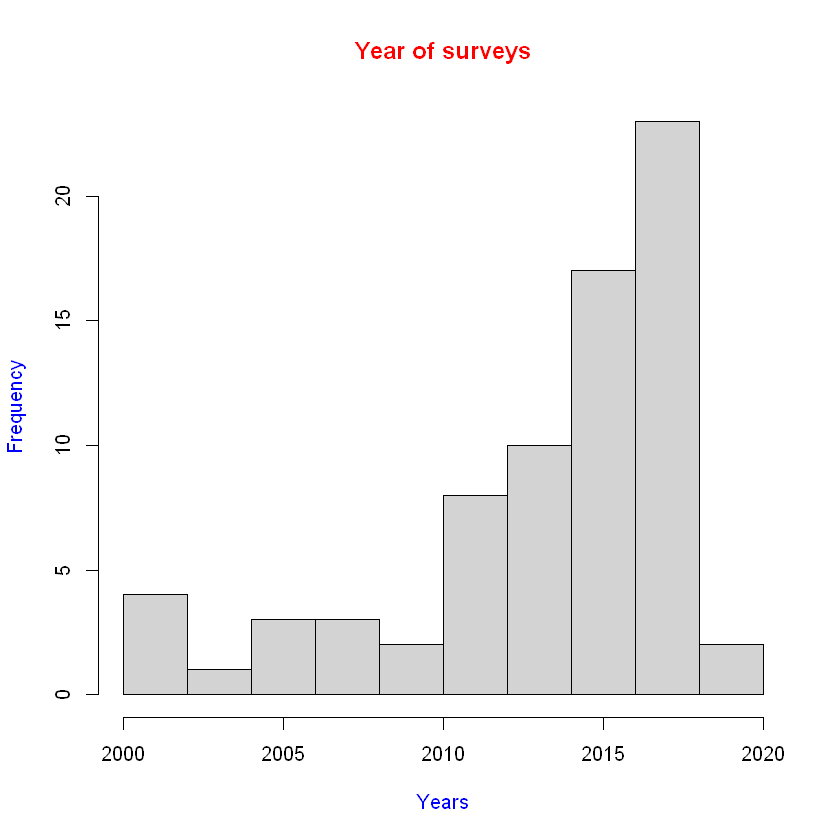
\includegraphics[width=.7\textwidth]{year}
  \caption{Distribution of years of water accessibility variables}
  \label{fig:year}
\end{figure}


\section{Methods}

\subsection{Preamble}
We analyzed data from the Demographic Health Survey (DHS) and the Malaria Indicator Survey (MIS) (1990-2020) to highlight water accessibility predictors in 78 countries throughout the world.

\subsection{Cluster analysis}
We elected 11 variables that describe water accessibility of 78 countries around the world \citep{price2019difference}. Next, we decided to implement clustering which is an unsupervised machine learning method to identify and group water accessibility variables in large data set to understand and make inferences about particular water accessibility variables. All of the clustering analysis was assisted by using the R program. Clustering ultimately can continue to assist in discovering the water accessibility predictor variables. 

First, we used a different clustering algorithm to determine the best clustering results. We tested and categorized differently by using single, average, complete, ward.D, and ward.D2 methods to develop clustering dendrogram. Then, we analyzed by determining the best hierarchical relationship of each of the methods by observing the tree diagram itself; if it has more of even distribution of each tree are the optimal clustering methods. We determined that ward.d2 had the best visual and even distribution, but to check this further, we used a function in R called 'NBClust' to determine the best algorithm as well as the best cut or groupings for the clustering methods as shown in \autoref{fig:optimal-clusters}. 

We compared Ward.D2, Ward.D, complete, and k-means algorithm methods to determine the best cuts, and also to confirm that Ward.D2 was the best clustering algorithm method to develop the deprogram tree. The 'NBClust' function was set to determine the best clustering methodology by choosing minimum clustering from 3 to max cuts of 7 and utilized all the indices.  The majority rule was implemented by the 'NBClust' function for Ward.d2, Ward.D, and the complete algorithm determined that the best clustering cut was four. However, k-means determined to be 3, but we determined that Ward.D2 is the best methodology thus far. 

Next, we compared the best indices values for different algorithm solving methodology to determine the best cuts to confirm that Ward.D2 is the best methodology. Once again, we determined that Ward.D2 was the best algorithm and learned that the best cut is four trees by analyzing within the different indices values of different algorithm theories. We compared the values by choosing KL, Ratkowsky, and Marriot values to compare what is the best cut for different clustering methods as shown in \autoref{fig:optimal}. 

\begin{table}[h!]
  \centering
  \begin{tabular}{p{1in} p{1in} p{1in}}\toprule
    \bf Methods & \bf KL (clusters) & \bf Value Index \\\midrule
    \texttt{Ward.D2} & 4 & 2.4982 \\\midrule
    \texttt{Ward.D} & 4 & 3.3397 \\\midrule
    \texttt{Complete} & 4 & 3.9093 \\\midrule
     \texttt{K-Means} & 12 & 8.6836  \\\bottomrule
  \end{tabular}
   \centering
  \begin{tabular}{p{1in} p{1in} p{1in}}\toprule
    \bf Methods & \bf Ratkowsky (clusters) & \bf Value Index \\\midrule
    \texttt{Ward.D2} & 4 & 0.2981 \\\midrule
    \texttt{Ward.D} & 4 & 0.2981 \\\midrule
    \texttt{Complete} & 3 & 0.3193 \\\midrule
     \texttt{K-Means} & 3 & 0.2948 \\\bottomrule
  \end{tabular}
   \centering
  \begin{tabular}{p{1in} p{1in} p{1in} p{1in} p{1in}}\toprule
    \bf Methods & \bf Marriot(clusters) & \bf Value Index & \bf Gap & \bf Majority Rule  \\\midrule
    \texttt{Ward.D2} & 4 & 1.54E+40 &  8 & 4 \\\midrule
    \texttt{Ward.D} & 4 & 1.79E+40 & 8 & 4 \\\midrule
    \texttt{Complete} & 4 & 1.77E+40  & 7 & 4 \\\midrule
     \texttt{K-Means} & 4 & 1.54E+40  & \texttt{N/A} & 3  \\\bottomrule
  \end{tabular}
  \caption{Summary of optimal clustering index values (Different Clustering Methods)}
  \label{tab:summary-optimal}
\end{table}

\autoref{tab:summary-optimal} is a rough summary of why Ward.D2 is the best clustering methodology if we go by four cuts. For the KL cluster algorithm, we determined that the best Value index is 2.4982 which is the lowest for the index, and the KL algorithm determines that the lowest value index results from the best cut of four. Also, the Ratkowsky cluster theorem determined that Ward.D2 was the best method for four cuts because the value index was the lowest matching Ward.D at .2981. However, Ward.D is the incomplete version of Ward.D2 where they forgot to square one of the intermediate value in the theorem. Therefore, Ward.D2 is the best clustering method for Ward.D2. Similarly, for the Marriot clustering theorem, Ward.D2 is the best once again due to the Ward.D having the greatest value index which determines that it is the best clustering method. Similar to an explanation from Ratkowsky, Ward.D2 is chosen to be the best method for 4 cuts. \autoref{fig:optimal} shows the visual representation of the explanation by the \autoref{tab:summary-optimal}. 

Lastly, we developed a horizontal dendrogram using R focusing on Ward.D2 methodology for clustering. We also cut the dendrogram in 4 trees as an 'NBClust' analysis as shown in \autoref{fig:dendrogram}. The clustering trees can be further be analyzed and the results and analysis will be discussed in the results and discussion section. 



\subsection{Classification model to explain water accessibility predictors}
\hl{This is the second phase of the work, which you should hopefully start in January}


\section{Results and Discussion}

\subsection{Model results}
First, we developed a correlation chart to quickly analyze if there is any great correlation between all the 28 numerical variables that may pertain to water accessibility. We recognized the strong and weak relationship by the size and color of the correlation plot is shown in \autoref{fig:cor-basic}, which indicates households with limited water service (liws) has the strongest and positive relationship with Households possessing a bicycle (bicy). Meanwhile, households using an improved water source (imws) has the strongest and negative relationship with households using an unimproved water source (uiws). This initial finding results indicated that the initial variables are logical and can give us insight into further understanding and the relationship between these variables. 

\begin{figure}[h!]
  \centering
  \includegraphics[width=.7\textwidth]{correlation-basic}
  \caption{Correlation Graph of Numerical Variables}
  \label{fig:cor-basic}
\end{figure}
As we continued to study further upon the correlations of the variables, we used more advanced correlation graphs to determined their p-value, and to see a relationship between different categorical variables is shown in \autoref{fig:cor-plot}, which again indicates a greater detailed comparison between the variables. Households with an improved water source on the premises (iwsp) have a strong relationship with households with basic water service (basw) of .84 and a p-value of less than 0.001. Also, we learned and discovered that Households using an unimproved water source (uiws) have a positive relationship with Households using unprotected well water (uwel), Households using an unprotected spring (uspr), and Households using surface water (surw) with a p-value of less than 0.001 as well. These relationships justify the necessity to research further if the particular water accessibility variables can increase the accessibility of particular water sources to reach universal access to water by 2030, as proposed in the SDGs. 



\begin{figure}[h!]
  \centering
  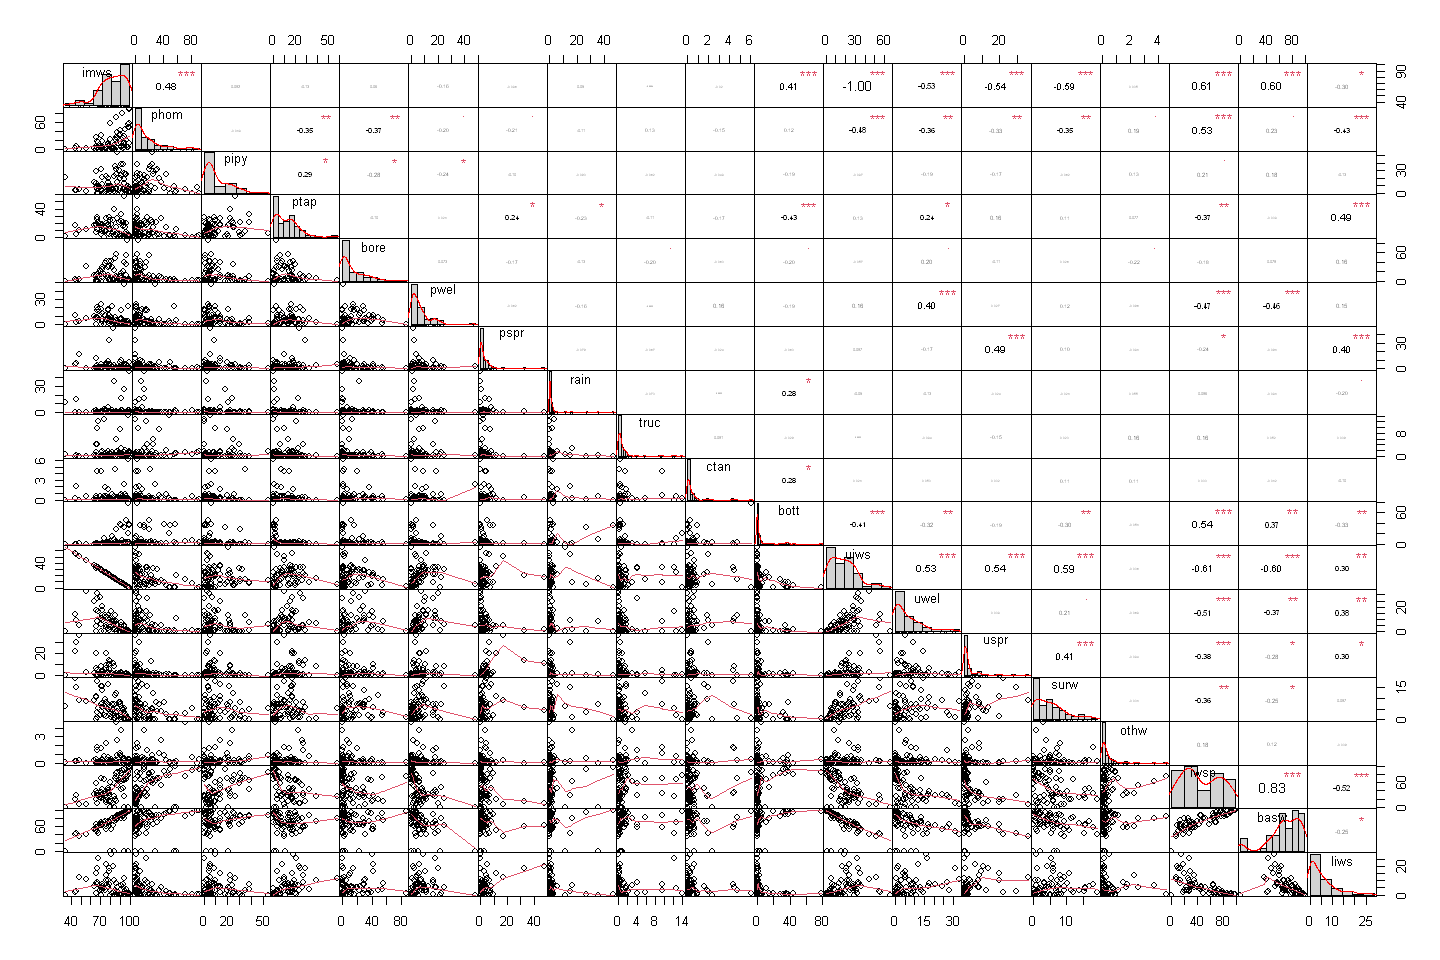
\includegraphics[width=.7\textwidth]{adv-cor-plot}
  \caption{Advanced Correlation Graph of Numerical Variables}
  \label{fig:cor-plot}
\end{figure}
Additionally, we wanted to explore if the modes of transportation variables have any relationship with potential water variables. Therefore, we investigated by developing more correlation plots relating transportation variables with water accessibility variables which are shown in \autoref{fig:transporation-time}, \autoref{fig:transporation-water-one}, \autoref{fig:transporation-water-two}. There is a significant positive relationship between households possessing a private car (pcar) and households with water on the premises (watp) as shown in \autoref{fig:transporation-time}. There is also is a significant negative relationship between households possessing a private car (pcar) with households with water 30 minutes or less away round trip (tles) and households with water more than 30 minutes away round trip (tmor) with a p-value of less than 0.001. This information is essential to investigate further why this is the global trend. 


\begin{figure}[h!]
  \centering
  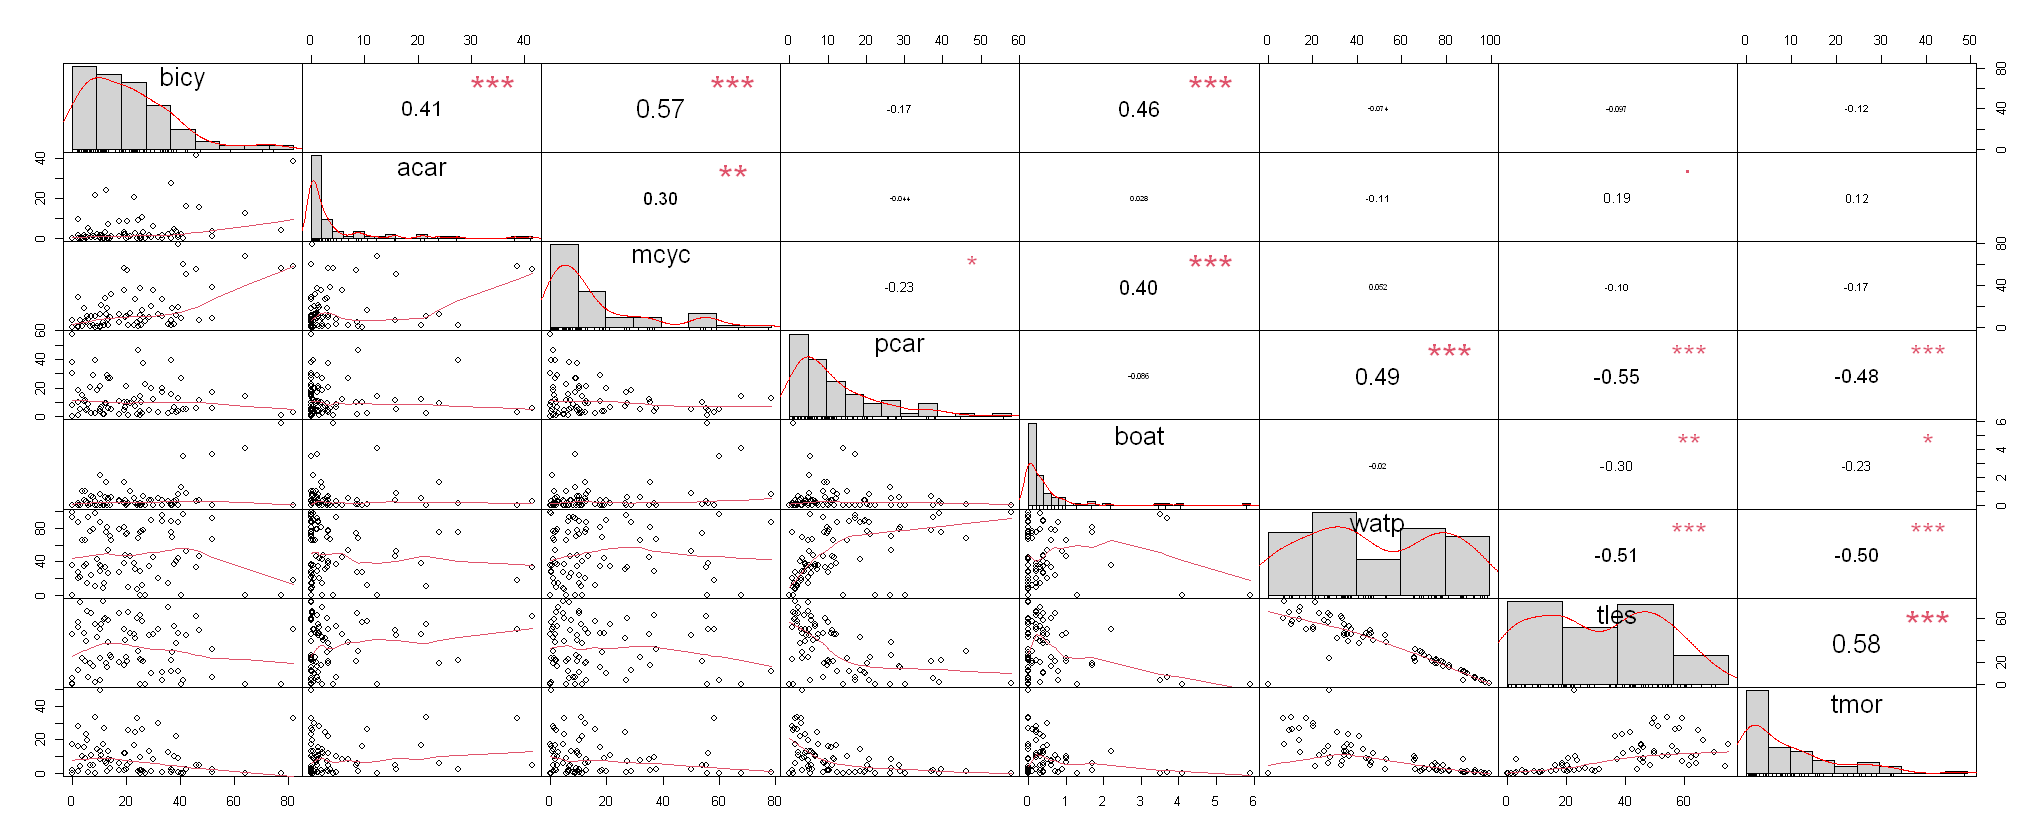
\includegraphics[width=.7\textwidth]{transportation-time}
  \caption{Advanced Correlation Graph of Modes of Transportation and Time}
  \label{fig:transporation-time}
\end{figure}
\autoref{fig:transporation-water-one} shows that Households possessing a motorcycle (mcyc) has a positive correlation with Households using a tube well/borehole (bore) and Households using rainwater (rain) with a p-value of less than 0.01. Similar to the previous analysis, there is a relationship between a mode of transportation to retrieve potential water sources. \autoref{fig:transporation-water-two} also shows that households possessing an animal-drawn cart (acar) have a positive and strong relationship with households using unprotected well water (uwel) with a p-value of less than 0.001. The results demonstrate that different modes of transportation factor into the accessibility of retrieving water sources on a global scale, therefore, there should be consideration of these variables to increase access to improved water sources. 
\begin{figure}[h!]
  \centering
  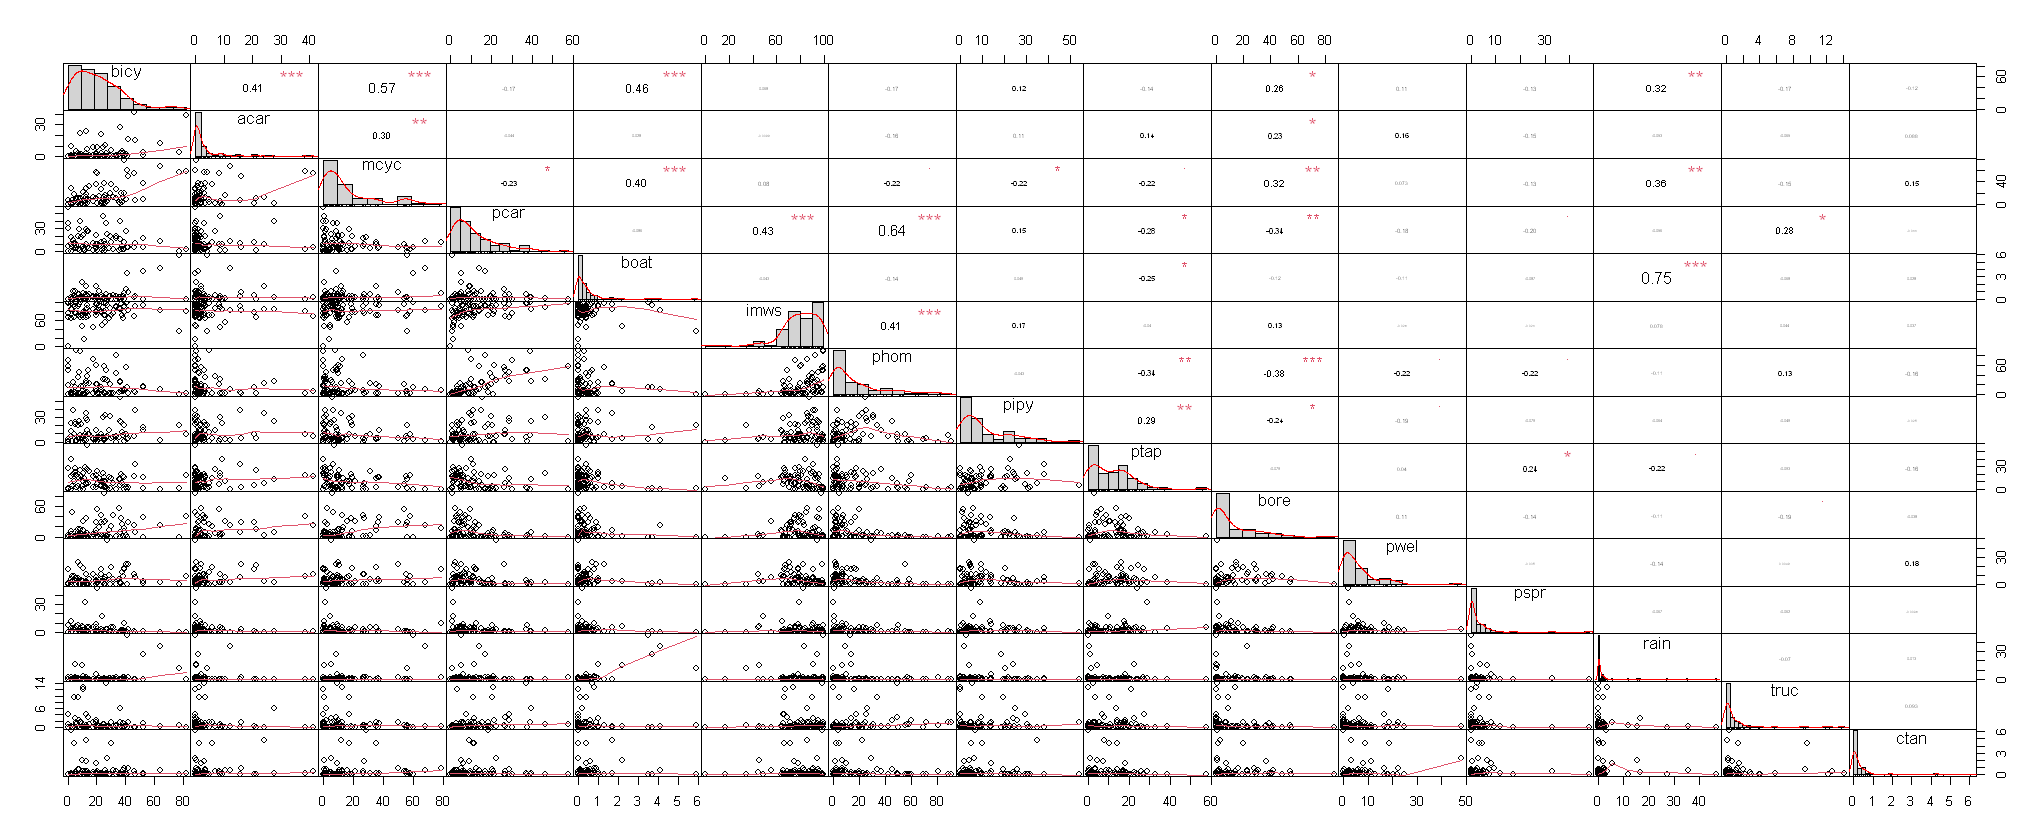
\includegraphics[width=.7\textwidth]{transportation-water-1}
  \caption{Advanced Correlation Graph of Modes of Transportation and Water Resources}
  \label{fig:transporation-water-one}
\end{figure}

\begin{figure}[h!]
  \centering
  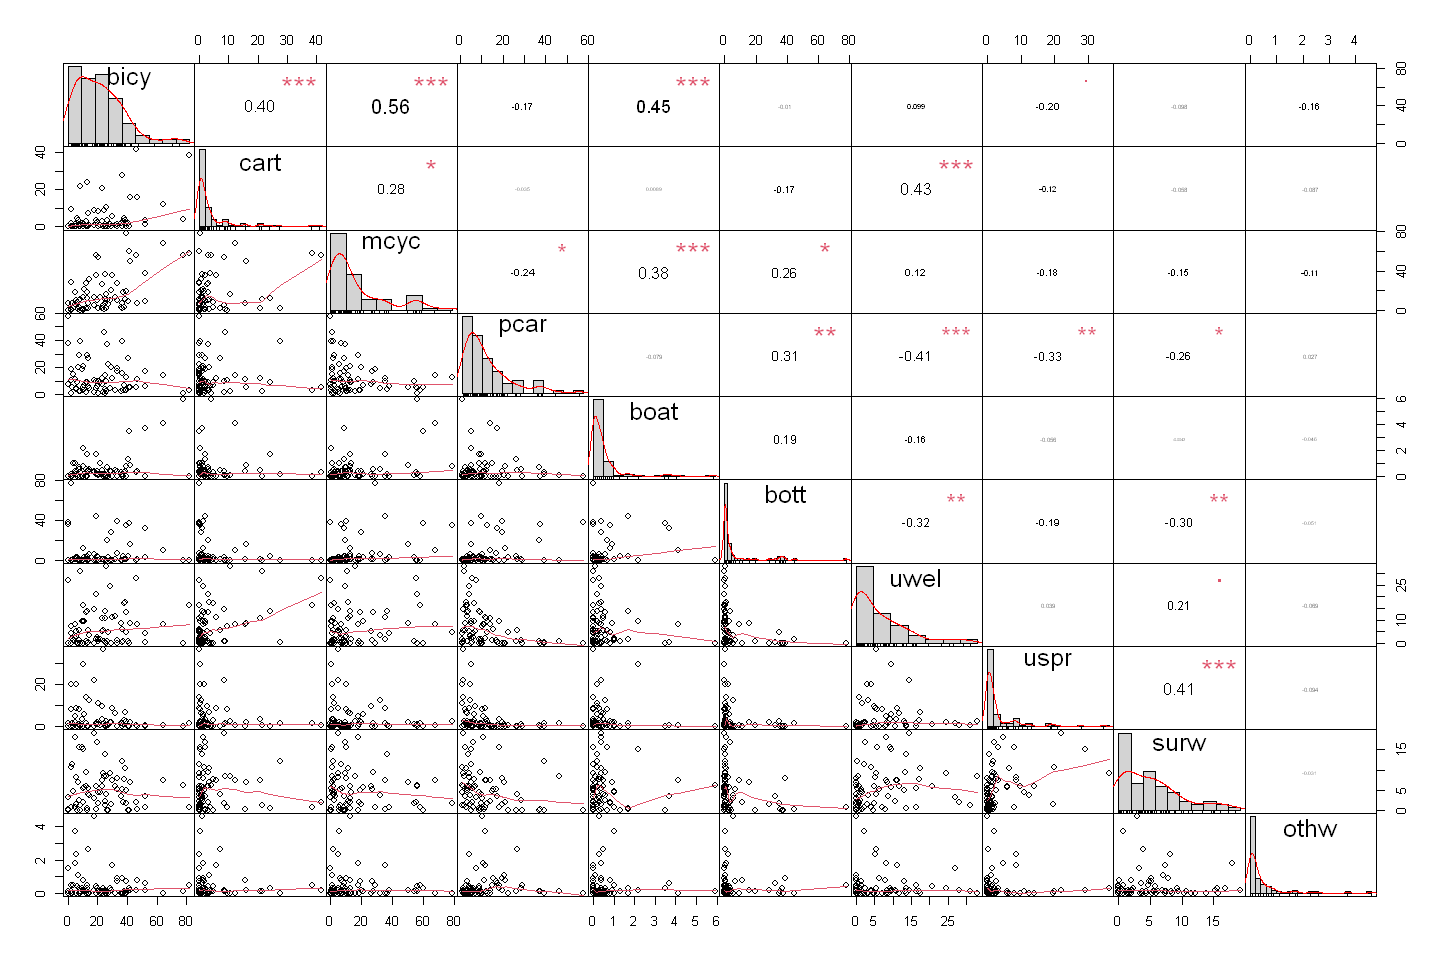
\includegraphics[width=.7\textwidth]{transportation-water-2}
  \caption{Advanced Correlation Graph of Modes of Transportation and Additional Water Resources}
  \label{fig:transporation-water-two}
\end{figure}

There is a problem of people not available to retrieve water quickly and there is a collection burden which is necessary to increase the water quality to improve many people's health and quality of life \citep{cassiviAccessDrinkingWater2018}. These initial findings can allow us to research into what are the major factors of water accessibility for the 76 countries by developing clustering and determining the water accessibility variable predictors. A future study could use the water accessibility variable predictors to implement policies and experiment if it improved water accessibility for the community. This would be a necessary implementation to invest to improve their access to water to reach universal access by 2030.



\subsection{Water accessibility typologies}

\hl{Show the typology/cluster results and discuss.}
NBClust statistic analysis developed and determined four distinct groups. The first cluster group is composed of countries near the equator or in the Sub-Sahara Regions. The analysis of the second group represents countries considered developed or recently industrialized. The third cluster group represents most of the countries in central Africa and may have similar factors as the first cluster group. The fourth cluster group represents most of the countries in the middle east or predominately non-African countries. There are great internally heterogeneous clusters for the 76 distinct countries. The cluster analysis' dendrogram is shown in \autoref{fig:dendrogram}, and the corresponding NBClust curve yielding the optimal four clusters is shown in \autoref{fig:optimal-clusters}, \autoref{fig:optimal}. \autoref{tab:water-cluster} shows the resulting four water accessibility country clusters. The cluster's water accessibility variables are summarized in \autoref{tab:summary-wa}. Through the optimal analysis of the clusters, which indicated the superior grouping of four cuts along with the relevant indicators. 

%    Fig. 3 shows the cluster country membership on a world map. 
\begin{table}[h!]
  \centering
  \begin{tabular}{p{1in} p{3in} }\toprule
    \bf Clusters & \bf Country Members \\\midrule
    \texttt{A (n=22)} & Afghanistan, Bangladesh, Benin, Burkina Faso, Cameroon, Chad, Ivory Coast, Ghana, Guinea, India, Liberia, Malawi, Mali, Myanmar, Nepal, Niger, Nigeria, Pakistan, Togo, Uganda, Zambia, Zimbabwe  \\\midrule
    \texttt{B (n=14)} & Albania, Armenia, Brazil, Colombia, Egypt, Honduras, Jordan, Kazakhstan, Morocco, Peru, South Africa, Turkey, Ukraine, Uzbekistan  \\\midrule
    \texttt{C (n=20)} & Angola, Burundi, Central African Republic, Congo, Congo Democratic Republic, Eritrea, Eswatini, Ethiopia, Gambia, Haiti, Kenya, Lesotho, Madagascar, Mauritania, Mozambique, Papua New Guinea, Rwanda, Sao Tome and Principe, Sierra Leone, Tanzania  \\\midrule
     \texttt{D (n=22)} & Azerbaijan, Bolivia, Cambodia, Comoros, Dominican Republic, Gabon, Guatemala, Guyana, Indonesia, Kyrgyz Republic, Maldives, Moldova, Namibia, Nicaragua, Paraguay, Philippines, Senegal, Tajikistan, Timor-Leste, Turkmenistan, Vietnam, Yemen  \\\bottomrule
  \end{tabular}
    \caption{Water accessibility country clusters.)}
  \label{tab:water-cluster}
\end{table}

	
\begin{figure}[h!]
  \centering
  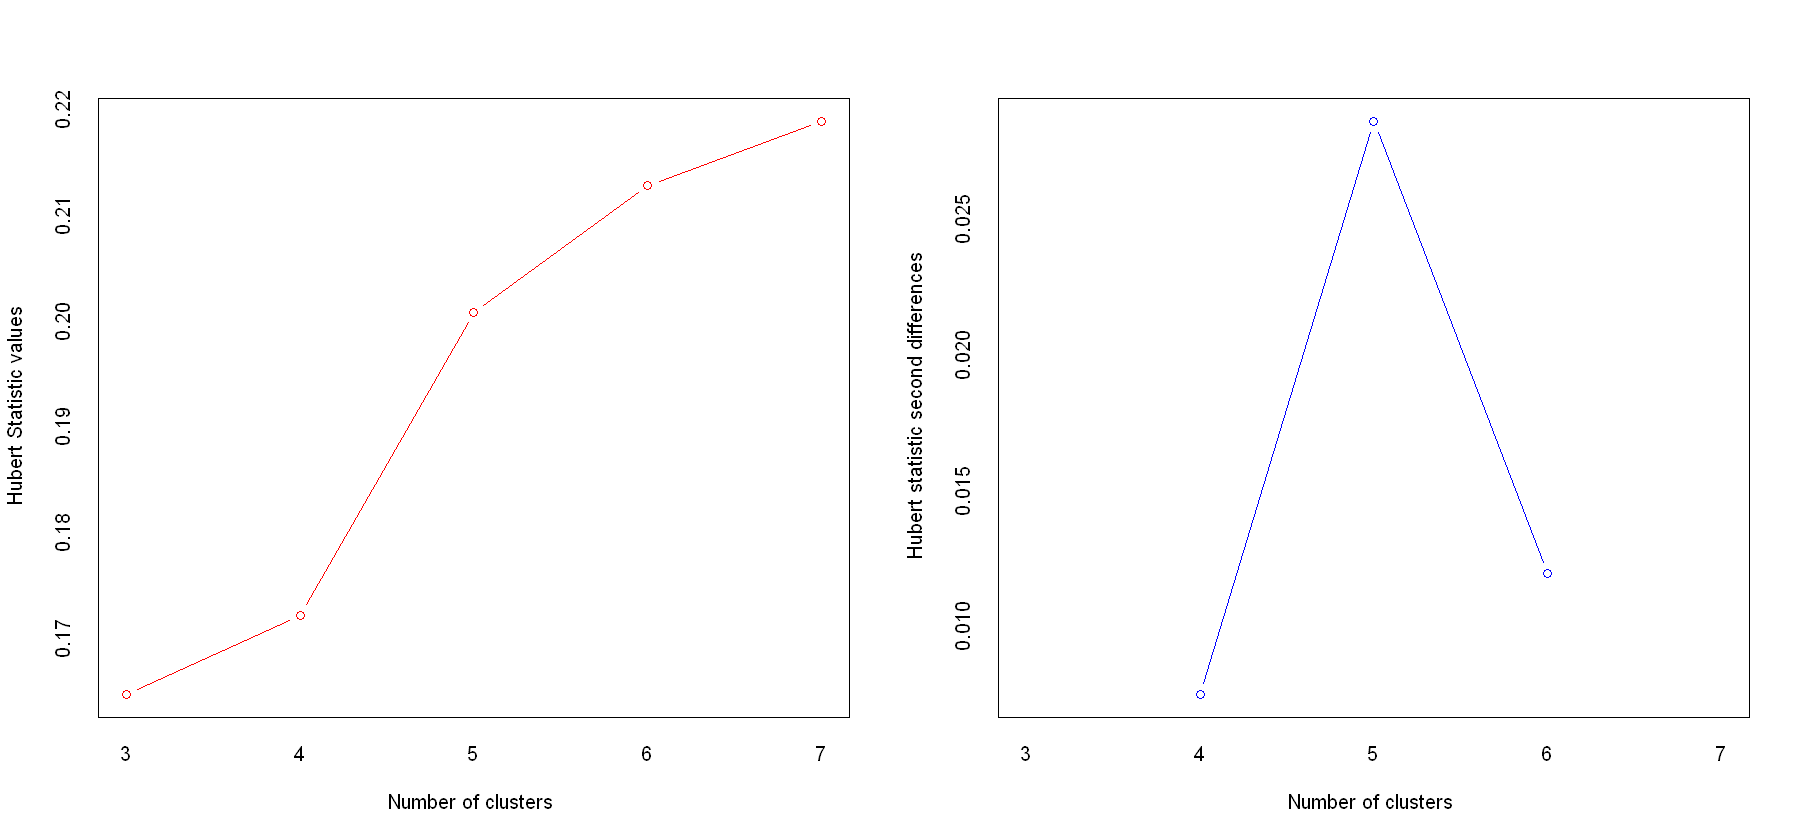
\includegraphics[width=.7\textwidth]{optimal-clusters-ward-d2}
  \caption{Optimal Number of Clusters for Ward.D2}
  \label{fig:optimal-clusters}
\end{figure}

\begin{figure}[h!]
  \centering
  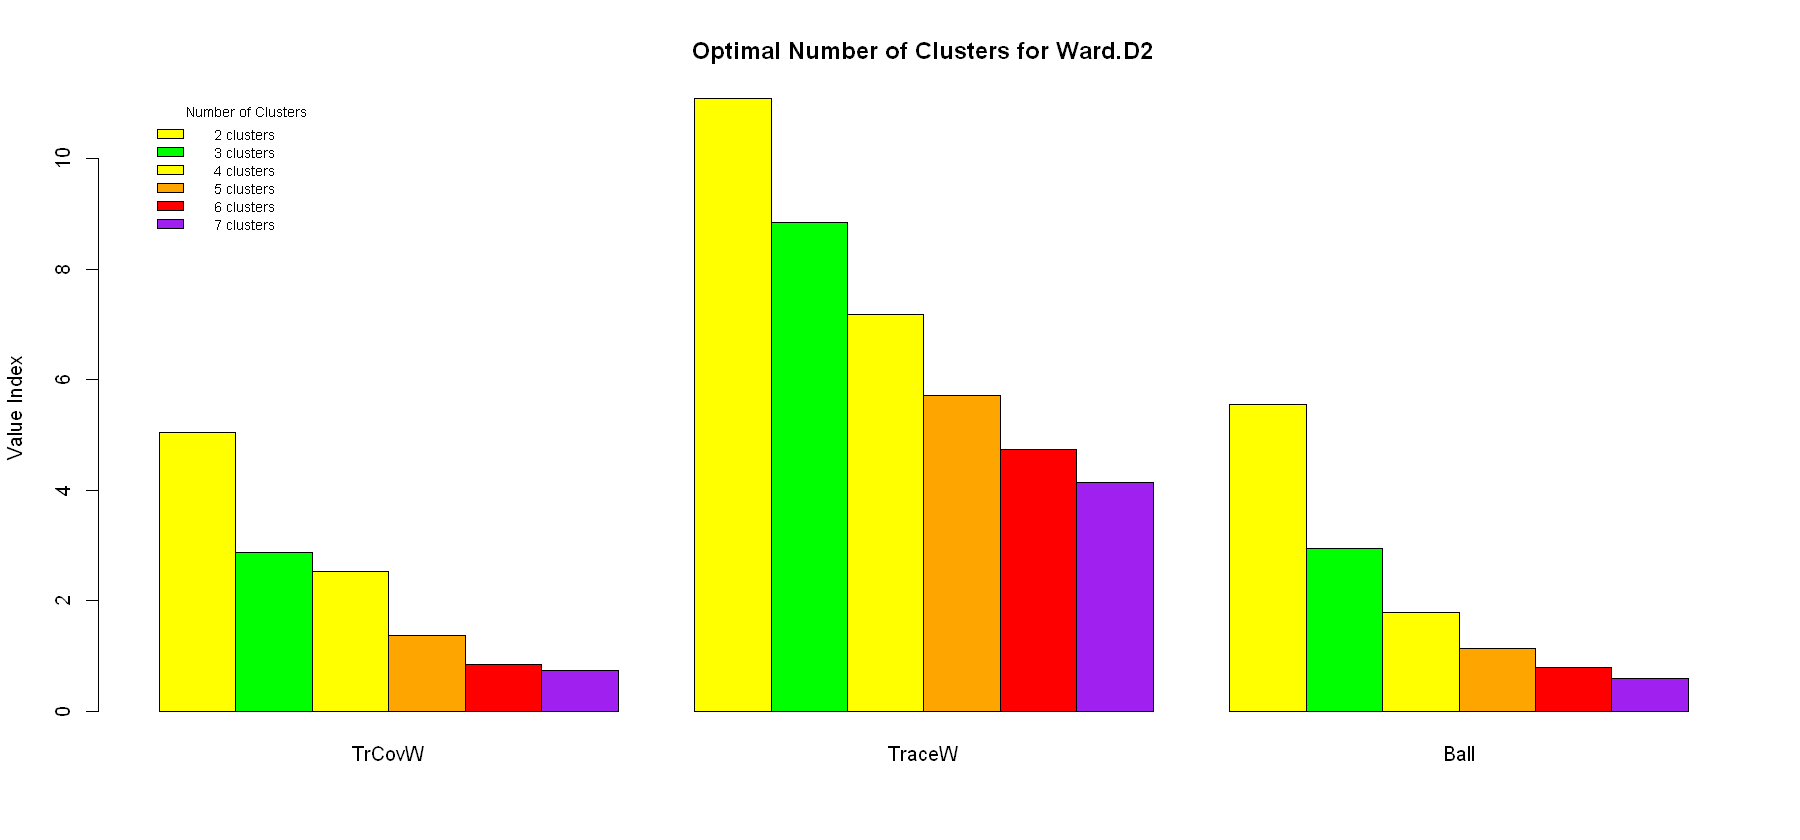
\includegraphics[width=.7\textwidth]{optimal-cuts}
  \caption{Optimal Number of Clusters for Ward.D2}
  \label{fig:optimal}
\end{figure}

\begin{figure}[h!]
  \centering
  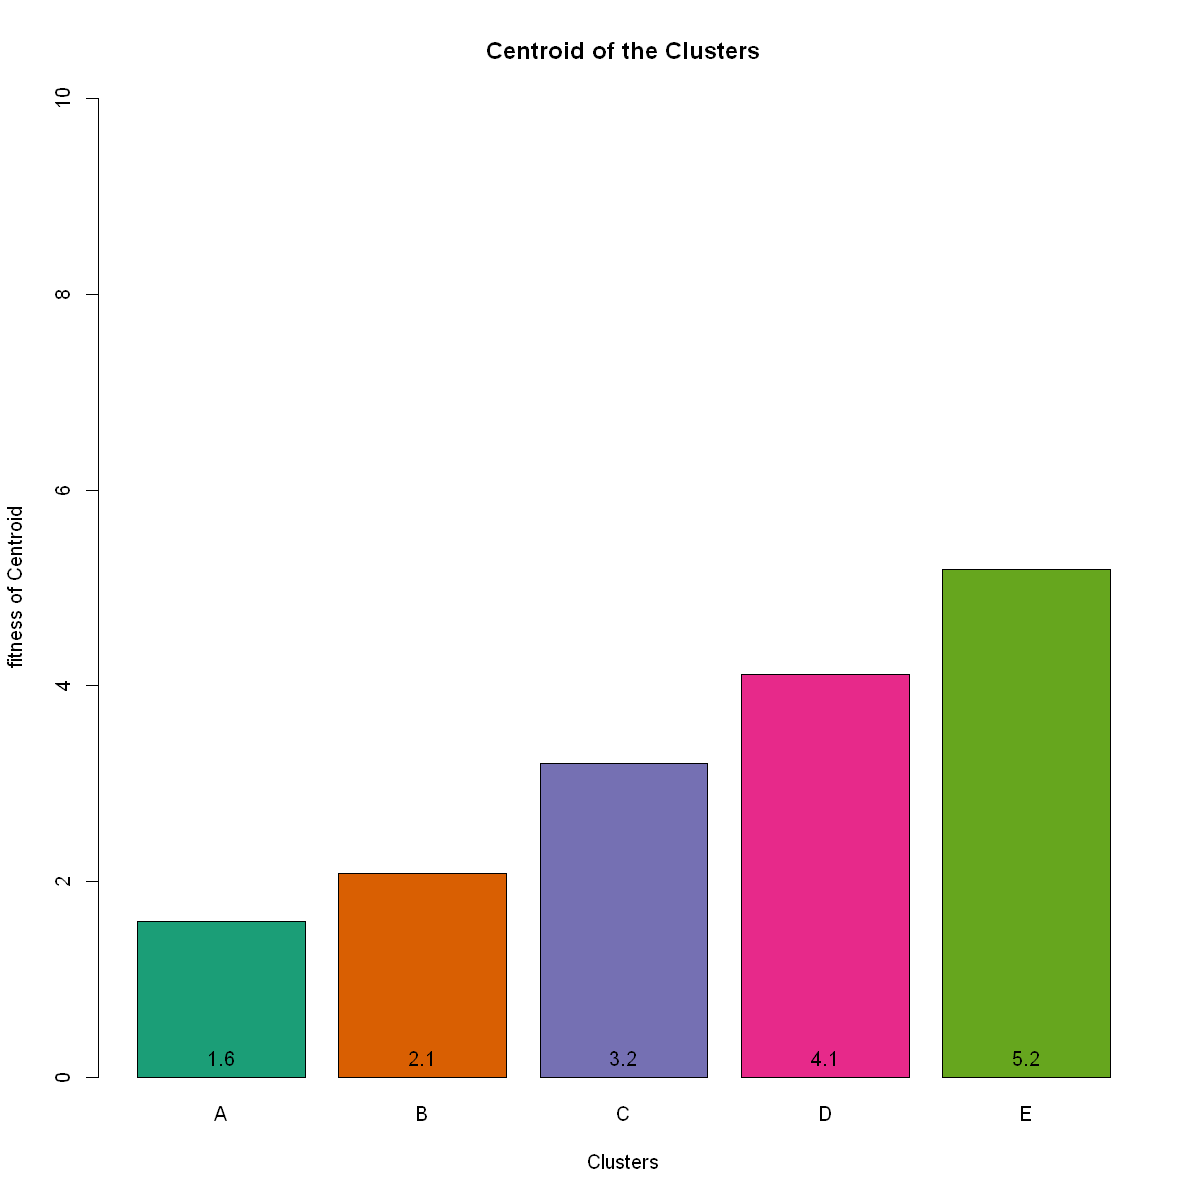
\includegraphics[width=.7\textwidth]{centroid}
  \caption{Centroid of the Four Cluster Groupings}
  \label{fig:centroid}
\end{figure}
\begin{figure}[h!]
  \centering
  \includegraphics[width=1\textwidth]{typology}
  \caption{Cluster Typology Average of Water Accessibility Variables }
  \label{fig:typology}
\end{figure}
\begin{figure}[h!]
\raggedright
  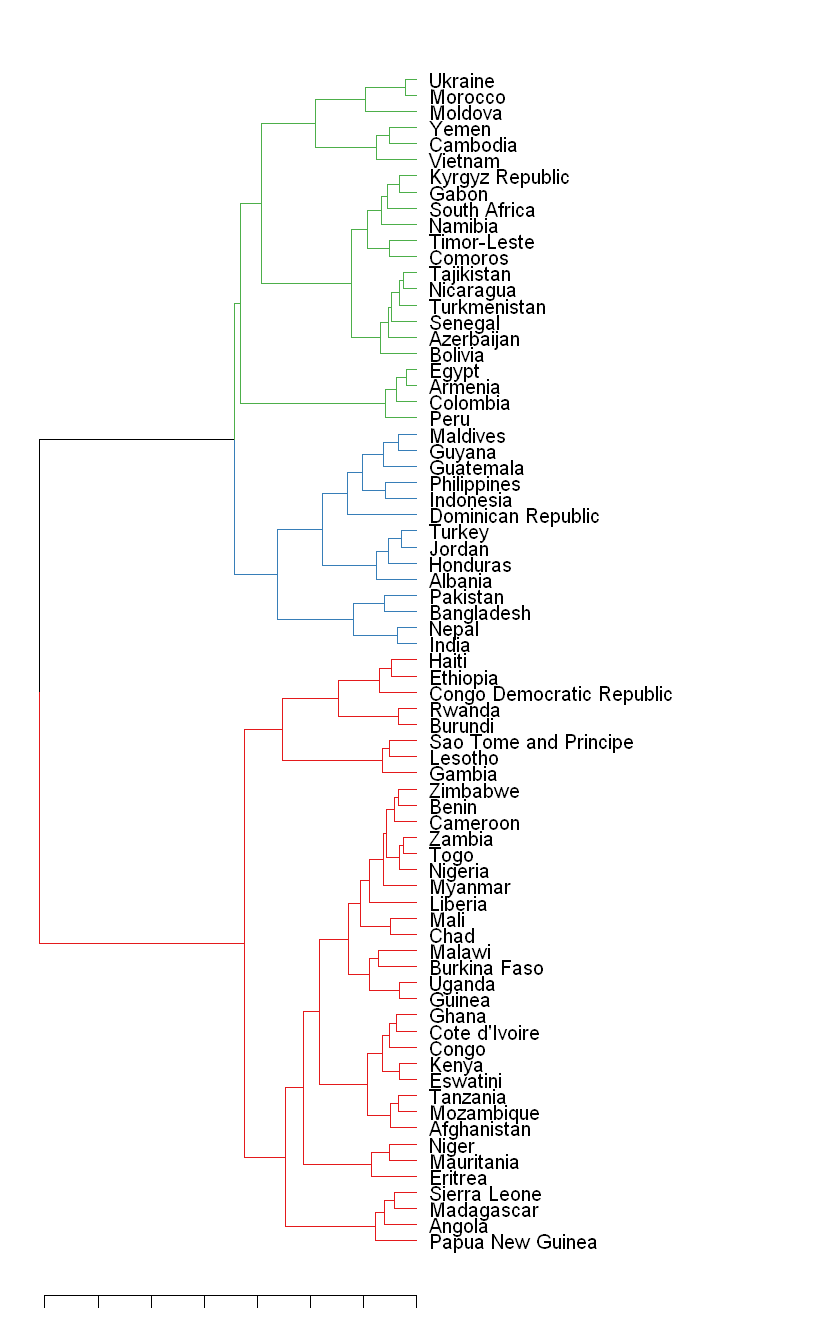
\includegraphics[width=1.1\textwidth]{dendrogram}
  \caption{Cluster Dendrogram with Four Cuts}
  \label{fig:dendrogram}
\end{figure}

\begin{figure}[h!]
  \centering
  \includegraphics[width= 1.25\textwidth]{spider-plot}
  \caption{Spider Plot of Water Accessibility Variables by Typology}
  \label{fig:spider}
\end{figure}

\subsection{Model results}
Cluster A consists of 22 countries with great cluster typology factor for Water 30 minutes or less away round trip (tles) 

%

  % \section*{Discussion}

\section{Conclusion}

\section{Limitation}
%he problem of missing data is relatively common in almost all research and can have a significant effect on the conclusions that can be drawn from the data.

\printbibliography

\end{document}

%%% Local Variables:
%%% mode: latex
%%% TeX-master: t
%%% End:
